\documentclass[11pt, aspectratio=169]{beamer}

\usepackage{amsmath, amsfonts, microtype, nicefrac, amssymb, amsthm, centernot}

\usepackage{pgfpages}

\usepackage{helvet}
\usepackage[default]{lato}
\usepackage{array}

\usefonttheme[onlymath]{serif}

\usepackage[utf8]{inputenc}
\usepackage[T1]{fontenc}
\usepackage{textcomp}
\usepackage{bm}

\usepackage{mathpazo}
\usepackage{hyperref}
\usepackage{multimedia}
\usepackage{graphicx}
\usepackage{multirow}
\usepackage{graphicx}
\usepackage{dcolumn}
\usepackage{bbm}
\newcolumntype{d}[0]{D{.}{.}{5}}

\usepackage{graphicx}
\usepackage[space]{grffile}
\usepackage{booktabs}

\usepackage{setspace}

\usepackage{transparent}


%%% FIGURES %%%
\usepackage{caption, subcaption}
\usepackage{booktabs, siunitx}
\usepackage{pgfplots} 
%\usepackage[outdir=./figures]{epstopdf}
\usepackage{float}
\usepackage{graphicx}
\usepackage[absolute, overlay]{textpos}
\usepackage{epstopdf}


%%% TIKZ %%%
\usepackage{tikz}
\usepackage{verbatim}
\usetikzlibrary{arrows.meta}
\usetikzlibrary{positioning}
\usetikzlibrary{bending}
\usetikzlibrary{snakes}
\usetikzlibrary{calc}
\usetikzlibrary{arrows}
\usetikzlibrary{decorations.markings}
\usetikzlibrary{shapes.misc}
\usetikzlibrary{matrix, shapes, arrows, fit, tikzmark}


%%% ALGORITHM %%%
\usepackage{algorithm}
\usepackage[noend]{algpseudocode}
\usepackage{multimedia}


%%% APPENDIX SLIDE NUMBERING %%%
\usepackage{appendixnumberbeamer}


%%% BEAMER BUTTON %%%
%\setbeamertemplate{button}{\tikz
	%\node[
	%	inner xsep = 2pt, 
	%	draw = structure!0, 
	%	fill = myblue, 
	%	rounded corners = 4pt]{\color{white} \tiny\insertbuttontext};
	%}


%%% COLORS %%%
\definecolor{blue}{RGB}{0,38,118}
\definecolor{red}{RGB}{213,94,0}
\definecolor{yellow}{RGB}{240,228,66}
\definecolor{green}{RGB}{0,158,115}

\definecolor{myred}{RGB}{163,32,45}
\definecolor{navyblue}{rgb}{0.05,0.2,0.70}
\definecolor{myblue}{RGB}{0,51,150}
\definecolor{myorange}{RGB}{255,140,0}
\definecolor{myref}{RGB}{160,160,160}
\definecolor{shock}{RGB}{0, 125, 34}%{50, 168, 82}

\definecolor{background}{RGB}{255,253,218}

% Define a new transparent color
\definecolor{trans}{rgb}{1,1,1}
\colorlet{trans}{black!20} % 0 percent opacity

\hypersetup{
  colorlinks=false,
  linkbordercolor = {white},
  linkcolor = {blue}
}

\setbeamercolor{frametitle}{fg=blue}
\setbeamercolor{title}{fg=black}
\setbeamertemplate{footline}[frame number]
\setbeamertemplate{navigation symbols}{} 
\setbeamertemplate{itemize items}{-}
\setbeamercolor{itemize item}{fg=blue}
\setbeamercolor{itemize subitem}{fg=blue}
\setbeamercolor{enumerate item}{fg=blue}
\setbeamercolor{enumerate subitem}{fg=blue}
\setbeamercolor{button}{bg=background, fg=blue,}

%\setbeamercolor{background canvas}{bg=background}


%%% FRAME TITLE %%%
\setbeamerfont{title}{series=\bfseries, parent=structure}
\setbeamerfont{frametitle}{series=\bfseries, parent=structure}


%%% TRANSITION FRAME %%%
\newenvironment{transitionframe}{
	\setbeamercolor{background canvas}{bg=blue}
	\begin{frame}
		\thispagestyle{empty}
		\addtocounter{framenumber}{-1}
		\vspace{42mm}
		\hspace{4mm} }{
		\begin{tikzpicture}
			\tikz \fill [white] (1,6) rectangle (20,10);
		\end{tikzpicture}
	\end{frame}
}


%%% OUTLINE %%%
\AtBeginSection[]
{
	\begin{frame}
       \frametitle{Roadmap of Talk}
       \tableofcontents[currentsection]
   \end{frame}
}
\setbeamercolor{section in toc}{fg=blue}
\setbeamercolor{subsection in toc}{fg=red}
\setbeamersize{text margin left=1em,text margin right=1em} 


%%% ENVIRONMENTS
\newenvironment{witemize}{\itemize\addtolength{\itemsep}{10pt}}{\enditemize}

\makeatother
\setbeamertemplate{itemize items}{\large\raisebox{0mm}{\textbullet}}
\setbeamertemplate{itemize subitem}{\footnotesize\raisebox{0.15ex}{--}}
\setbeamertemplate{itemize subsubitem}{\Tiny\raisebox{0.7ex}{$\blacktriangleright$}}

\setbeamertemplate{enumerate item}[default]
\setbeamertemplate{enumerate subitem}{\textbullet}
\makeatletter

% ITEMIZE SPACING:
% \usepackage{xpatch}
% \xpatchcmd{\itemize}
% {\def\makelabel}
% {\setlength{\itemsep}{0mm}\def\makelabel}
% {}
% {}


%%% PRETTY ENUMERATE %%%
% \usepackage{stackengine,xcolor}
% \newcommand\circnum[2]{\stackinset{c}{}{c}{.1ex}{\small\textcolor{white}{#2}}%
	% 	{\abovebaseline[-.7ex]{\Huge\textcolor{#1}{$\bullet$}}}}
% \newenvironment{myenum}
% {\let\svitem\item
	% 	\renewcommand\item[1][black]{%
		% 		\refstepcounter{enumi}\svitem[\circnum{##1}{\theenumi}]}%
	% 	\begin{enumerate}}{\end{enumerate}}
\usepackage{stackengine,xcolor,graphicx}
\newcommand\circnum[2]{\smash{\stackinset{c}{}{c}{.2ex}{\small\textcolor{white}{#2}}%
		{\abovebaseline[-1.1ex]{\Huge\textcolor{#1}{\scalebox{1.5}{$\bullet$}}}}}}
\newenvironment{myenum}
{\let\svitem\item
	\renewcommand\item[1][black]{%
		\refstepcounter{enumi}\svitem[\circnum{##1}{\theenumi}]}%
	\begin{enumerate}}{\end{enumerate}}

\newcommand{\notimplies}{\;\not\!\!\!\implies}



%%%%%%%%%%%%%%%%%%%%%%%%%%  TITLE   %%%%%%%%%%%%%%%%%%%%%%%%%%%%%%%%
\title[]{\\[8pt]
	{\large \color{blue} Dynamic Programming and Applications \\[5pt] \normalfont{Consumption} \\[10pt] \normalfont{Lectures 7--8}}}
\author[Schaab]{Andreas Schaab}
\institute{}
\subject{}
\date{}



%%%%%%%%%%%%%%%%%%%%%%%%  BEGIN DOC   %%%%%%%%%%%%%%%%%%%%%%%%%%%%%%%
\begin{document}

%%% TIKZ %%% 
\tikzstyle{every picture}+=[remember picture]
%\everymath{\displaystyle}

\tikzset{   
	every picture/.style={remember picture,baseline},
	every node/.style={anchor=base,align=center,outer sep=1.5pt},
	every path/.style={thick},
}
\newcommand\marktopleft[1]{%
	\tikz[overlay,remember picture] 
	\node (marker-#1-a) at (-.3em,.3em) {};%
}
\newcommand\markbottomright[2]{%
	\tikz[overlay,remember picture] 
	\node (marker-#1-b) at (0em,0em) {};%
}
\tikzstyle{every picture}+=[remember picture] 
\tikzstyle{mybox} =[draw=black, very thick, rectangle, inner sep=10pt, inner ysep=20pt]
\tikzstyle{fancytitle} =[draw=black,fill=red, text=white]


\addtocounter{framenumber}{-1}
\thispagestyle{empty}
\maketitle 
\newpage



%%%%%%%%%%%%%%%%%%%%%%%%%%  SLIDE   %%%%%%%%%%%%%%%%%%%%%%%%%%%%%%%%
\begin{frame}{Outline}
\thispagestyle{empty}
\addtocounter{framenumber}{-1}

Part 1: Early theories of consumption
\begin{enumerate}
\item The old-Keynesian consumption function

\item The consumption Euler equation

\item The permanent income hypothesis (PIH)

\item The certainty equivalence model (Hall 1978)

\item Precautionary savings 

\item Linearization of the Euler Equation

\end{enumerate}

\end{frame}


%%%%%%%%%%%%%%%%%%%%%%%%%%  SLIDE   %%%%%%%%%%%%%%%%%%%%%%%%%%%%%%%%
\begin{frame}{Outline}
\thispagestyle{empty}
\addtocounter{framenumber}{-1}

Part 2: Empirical regularities 
\begin{enumerate}
\item Empirical tests of the consumption Euler equation

\item How does consumption move with income fluctuations?

\item What is the marginal propensity to consume (MPC) out of income?
\end{enumerate}

\vspace{5mm}
Part 3: Tractable models of consumption and MPCs
\begin{enumerate}
\item Eat-the-pie 
\item Unearned income 
\item Labor supply
\item Precautionary savings
\end{enumerate}

\vspace{5mm}
Part 4: The canonical consumption model with liquidity constraints

\end{frame}




%%%%%%%%%%%%%%%%%%%%%%%%%%  SLIDE   %%%%%%%%%%%%%%%%%%%%%%%%%%%%%%%%
\begin{transitionframe}
	{\color{white} \Huge \textbf{Part 1: Early Theories} \vspace{2mm}}
\end{transitionframe}


%%%%%%%%%%%%%%%%%%%%%%%%%%  SLIDE   %%%%%%%%%%%%%%%%%%%%%%%%%%%%%%%%
\begin{frame}{1. The old-Keynesian consumption function}

Keynes (1936, p. 96):
\begin{quote}
	The fundamental psychological law, upon which we are entitled to depend with great confidence both \textnormal{a priori} and from our knowledge of human nature and from detailed facts of experience, is that [people] are disposed, as a rule and on average, to increase their consumption as their income increases, but not by as much as the increase in their income.
\end{quote}

\vspace{5mm}
Keynes (1936, p. 93-94):
\begin{quote}
	The usual type of short-period fluctuation in the rate of interest is not likely, however, to have much \textnormal{direct} influence on spending either way. There are not many people who will alter their way of living because the rate of interest has fallen from 5 to 4 per cent, if their aggregate income is the same as before.
\end{quote}

\end{frame}




%%%%%%%%%%%%%%%%%%%%%%%%%%  SLIDE   %%%%%%%%%%%%%%%%%%%%%%%%%%%%%%%%
\begin{frame}{Keynes' Consumption Function}

\begin{equation*}
	C_t = \alpha + \gamma (Y_t - T_t) 
\end{equation*}

\begin{witemize}
	\item Consumption a function of after-tax income
	\item Marginal propensity to consume ($\gamma$) between zero and one
	\item Interest rates not important
	\item Future income not important
\end{witemize}
\end{frame}


%%%%%%%%%%%%%%%%%%%%%%%%%%  SLIDE   %%%%%%%%%%%%%%%%%%%%%%%%%%%%%%%%
\begin{frame}{Three Landmark Empirical Studies}

``dealt a fatal blow to this extraordinarily simple view of the savings process'' {\small (Modigliani 86)}

\vspace{10pt}
\begin{witemize}
	\item Simon Kuznetz (1946):
	\begin{itemize}
		\item National Income and Product Accounts back to 1899
		\item No rise in aggregate savings over time
	\end{itemize}
	\item Dorothy Brady and Rose D. Friedman (1947):
	\begin{itemize}
		\item Re-analyze budget study data 
		\item Consumption function shifts up over time as average income increases
	\end{itemize}
	\item Margaret Reid (unpublished):
	\begin{itemize}
		\item Re-analyzes budget study data
		\item Introduces concept of ``permanent component of income'' 
	\end{itemize}
\end{witemize}

\vspace{5pt}
{\small (See Burns (2022) for history of ``Hidden Figures.'')}

\end{frame}



%%%%%%%%%%%%%%%%%%%%%%%%%%  SLIDE   %%%%%%%%%%%%%%%%%%%%%%%%%%%%%%%%
\begin{frame}{2. Canonical model of consumption}

\begin{witemize}
\item Canonical model known as \textbf{consumption-savings} or \textbf{income-fluctuations} problem:
\begin{equation*}
	V(a_0) = \max_{ \{c_t\}_{t=0}^\infty } \, \mathbb{E}_0 \sum_{t=0}^\infty \beta^t u(c_t)
\end{equation*}
subject to
\begin{equation*}
	a_{t+1} = R_{t+1} (a_t - c_t) + y_t
\end{equation*}

\item $a_t$ is wealth, $R_{t+1}$ is deterministic (gross) interest rate and $y_t$ is iid. income risk

\item Assume $u(\cdot)$ concave ($u' > 0$ and $u''< 0$ for all $c$) and $\lim_{c \to 0} u'(c) = \infty$

\item What should we assume about borrowing capacity?
\begin{itemize}
\vspace{1mm}
\item Natural borrowing limit: $a_t \geq a^n$

\item Ad-hoc borrowing limit: $a_t \geq \underline a$
\end{itemize}

\end{witemize}
\end{frame}


%%%%%%%%%%%%%%%%%%%%%%%%%%  SLIDE   %%%%%%%%%%%%%%%%%%%%%%%%%%%%%%%%
\begin{frame}{}
\begin{itemize}
\item Bellman equation:
\begin{align*}
	V_t(a) &= \max_{c, a'} \Big\{ u(c) + \beta \mathbb{E}_t V_{t+1}(a') \Big\} \;\; s.t. \;\; a' = R_{t+1} (a - c) + y
\end{align*}

\item Bellman equation may not be stationary or time-independent: $R_t$

\item If income process $\{y_t\}$ persistent, would need $y$ as second state variable

\item First-order conditions (with ad-hoc borrowing limit $\underline a$):
\begin{align*}
	u'(c_t(a)) = &\; \beta R_{t+1} \mathbb{E}_t \frac{\partial V_{t+1}(a')}{\partial a'} \quad \text{ if }  a' > \underline a \\
	u'(c_t(a)) \geq &\; \beta R_{t+1} \mathbb{E}_t \frac{\partial V_{t+1}(a')}{\partial a'} \quad \text{ if }  a' = \underline a
\end{align*}

\end{itemize}
\end{frame}


%%%%%%%%%%%%%%%%%%%%%%%%%%  SLIDE   %%%%%%%%%%%%%%%%%%%%%%%%%%%%%%%%
\begin{frame}{}
\begin{itemize}
\item Envelope theorem: $\frac{\partial V_t(a)}{\partial a} = u'(c_t(a))$

\item So we again get a consumption Euler equation:
\begin{align*}
	u'(c_t) = &\; \beta R_{t+1} \mathbb{E}_t u'(c_{t+1}) \quad \text{ if }  a' > \underline a \\
	u'(c_t) \geq &\; \beta R_{t+1} \mathbb{E}_t u'(c_{t+1})  \quad \text{ if }  a' = \underline a
\end{align*}
\end{itemize}


\vspace{6mm}
Perturbation intuition:
\begin{itemize}
\item What is the cost of consuming $\epsilon$ dollars less today? 
\begin{equation*}
	\text{Utility loss today} = \epsilon \cdot u'(c_t)
\end{equation*}

\item What is the expected, discounted gain of consuming $\epsilon \cdot R_{t+1}$ dollars more tomorrow?
\begin{equation*}
	\text{Utility gain tomorrow} = \beta (\epsilon \cdot R_{t+1}) \mathbb{E}_t u'(c_{t+1})
\end{equation*}
\end{itemize}

\end{frame}



%%%%%%%%%%%%%%%%%%%%%%%%%%  SLIDE   %%%%%%%%%%%%%%%%%%%%%%%%%%%%%%%%
\begin{frame}{3. Permanent Income Hypothesis (PIH)}
\begin{itemize}
	\itemsep1em 
	\item Originally developed independently by:
	\begin{itemize}
		\item Modigiani and Brumberg (1954) (Life-Cycle Hypothesis)
		\item Friedman (1957) (Permanent Income Hypothesis)
	\end{itemize}
	\item Basic idea:
	\begin{itemize}
		\item Utility maximization and perfect markets imply that current \\ consumption is determined by net present value of life-time income
	\end{itemize}
	\item Dramatically different from Keynesian consumption function
\end{itemize}
\end{frame}


%%%%%%%%%%%%%%%%%%%%%%%%%%  SLIDE   %%%%%%%%%%%%%%%%%%%%%%%%%%%%%%%%
\begin{frame}{}
Life Cycle Hypothesis: Modigliani \& Brumberg (1954)
\vspace{3mm}
\begin{witemize}
\item $R_t = R$ for all $t$, and $\beta R = 1$

\item No assumption on (stochastic) income process $\{y_t\}$

\item Perfect capital markets (i.e., no moral hazard), so that future income, $y_t$, can be exchanged for current capital. Let's assume that your counter-party is risk neutral
\end{witemize}
\end{frame}


%%%%%%%%%%%%%%%%%%%%%%%%%%  SLIDE   %%%%%%%%%%%%%%%%%%%%%%%%%%%%%%%%
\begin{frame}{}

\textbf{Bellman Equation}:
\begin{equation*}
	v(x) = \max_{c \leq x} \Big\{u(c) + \beta v(x) \Big\} 
\end{equation*}
subject to
\begin{equation*}
	x' = R(x - c) 
	\quad\quad \text{ and } \quad\quad
	x_0 = \mathbb E \sum_{t=0}^\infty R^{-t} y_t
\end{equation*}

\vspace{3mm}
\begin{witemize}
\item Sometimes referred to as ``eating a pie/cake problem''

\item Euler Equation implies
\begin{equation*}
	u'(c_t) = \beta R u'(c_{t+1}) = u'(c_{t+1}) 
\end{equation*}

\item Hence, consumption is constant: $c_t = c_{t-1}$ regardless of $y_t$
\end{witemize}
\end{frame}


%%%%%%%%%%%%%%%%%%%%%%%%%%  SLIDE   %%%%%%%%%%%%%%%%%%%%%%%%%%%%%%%%
\begin{frame}{}

\begin{witemize}
\item Budget constraint:
\begin{equation*}
	\sum_{t=0}^{\infty} R^{-t} c_t = \mathbb E_0 \sum_{t=0}^{\infty} R^{-t} y_t 
\end{equation*}

\item Substitute Euler Equation, $c_0 = c_t$ to find 
\begin{equation*}
	\sum_{t=0}^{\infty} R^{-t} c_0 = \mathbb E_0 \sum_{t=0}^\infty R^{-t} y_t 
\end{equation*}

\item So Euler Equation + budget constraint implies 
\begin{equation*}
	c_0 = \bigg(1 - \frac{1}{R}\bigg) \mathbb E_0 \sum_{t=0}^\infty R^{-t} y_t
\end{equation*}

\item Consumption is an annuity. Note that $(1-\frac{1}{R}) \simeq (1-\frac{1}{1}) +\frac{1}{R_{|R=1}^{2}}(R-1)=R-1=r$

\end{witemize}
\end{frame}



%%%%%%%%%%%%%%%%%%%%%%%%%%  SLIDE   %%%%%%%%%%%%%%%%%%%%%%%%%%%%%%%%
\begin{frame}{4. Certainty Equivalence Model: Hall (1978)}

\begin{witemize}
\item $R_t = R$ for all $t$ and $\beta R = 1$

\item Quadratic utility: $u(c) = \alpha c - \frac{\gamma}{2} c^2$

\begin{itemize}
\item This admits negative consumption

\item And this does \textbf{not} imply $\lim_{c\downarrow 0} u'(c) = \infty$
\end{itemize}

\item Now assume you can't sell claims to labor income

\item No interest rate uncertainty, but household now bears exposure to stochastic income fluctuations
\end{witemize}
\end{frame}


%%%%%%%%%%%%%%%%%%%%%%%%%%  SLIDE   %%%%%%%%%%%%%%%%%%%%%%%%%%%%%%%%
\begin{frame}{}

\begin{witemize}
\item Euler Equation 
\begin{equation*}
	u'(c_t) = \beta R \mathbb E_t u'(c_{t+1}) 
\end{equation*}
implies, 
\begin{align*}
	- \gamma c_t &= -\gamma \mathbb E_t c_{t+1} \\
	c_t &= \mathbb E_t c_{t+1} = \mathbb E_t c_{t+n}.
\end{align*}
So consumption is a random walk (martingale): 
\begin{equation*}
	c_{t+1} = c_t + \eta_{t+1}. 
\end{equation*}

\item So $\Delta c_{t+1} \equiv c_{t+1} - c_t$ cannot be predicted by any information available
at time $t$
\end{witemize}

\end{frame}


%%%%%%%%%%%%%%%%%%%%%%%%%%  SLIDE   %%%%%%%%%%%%%%%%%%%%%%%%%%%%%%%%
\begin{frame}{}

\begin{witemize}
\item Budget constraint at date $t$ is (along any proceeding history)
\begin{equation*}
	\sum_{s=0}^\infty R^{-s} c_{t+s} = x_t + \sum_{s=1}^\infty R^{-s} y_{t+s} 
\end{equation*}
\begin{equation*}
	\hspace{-10mm} \implies \mathbb E_t \sum_{s=0}^\infty R^{-s} c_{t+s} = x_t + \mathbb E_t \sum_{s=1}^\infty R^{-s} y_{t+s} 
\end{equation*}

\item Substitute $c_t = \mathbb E_t c_{t+s}$:
\begin{equation*}
	\sum_{s=0}^\infty R^{-s} c_t = x_t + \mathbb E_t \sum_{s=1}^\infty R^{-s} y_{t+s}
\end{equation*}

\item So Euler Equation + budget constraint implies 
\begin{equation*}
	c_t = \bigg(1-\frac{1}{R}\bigg) \bigg(x_t + \mathbb E_t \sum_{s=1}^\infty
R^{-s} y_{t+s} \bigg) 
\end{equation*}

\end{witemize}
\end{frame}



%%%%%%%%%%%%%%%%%%%%%%%%%%  SLIDE   %%%%%%%%%%%%%%%%%%%%%%%%%%%%%%%%
\begin{frame}{5. Precautionary Savings}

\begin{witemize}
\item Recall certainty equivalence model:
\begin{equation*}
	c_t = \mathbb E_t c_{t + 1}
\end{equation*}


\item Imagine there are two periods, interest rate is 0 
\end{witemize}

\vspace{8mm}
\only<2>{
Scenario \textbf{A}:
\begin{witemize}
\item You get \$200 today
\item You get \$100 tomorrow with certainty
\item How much would you save today?
\end{witemize}
}

\only<3>{
Scenario \textbf{B}:
\begin{witemize}
	\item You get \$200 today as before
	\item You get \$200 tomorrow with probability $\frac{1}{2}$, and \$0 otherwise
	\item How much would you save today?
\end{witemize}
}

\end{frame}



%%%%%%%%%%%%%%%%%%%%%%%%%%  SLIDE   %%%%%%%%%%%%%%%%%%%%%%%%%%%%%%%%
\begin{frame}{}

\begin{witemize}
\item Curvature of utility almost surely falls as consumption rises:
\begin{equation*}
	u'''(c_t) > 0
\end{equation*}

\item This implies that marginal utility $u'(c_t)$ is convex

\item Suppose you currently consume such that $c_t = \mathbb E_t c_{t+1}$. Is this optimal?

\item Notice: $u'(c_t) = u'(\mathbb E_t c_{t+1}) < \mathbb E_t u'(c_{t+1})$

\item Therefore: marginally raising $c_t$ increases utility

\item This extra saving today (higher $c_t$) relative to certainty equivalence case is called \textbf{precautionary savings}

\end{witemize}
\end{frame}


%%%%%%%%%%%%%%%%%%%%%%%%%%  SLIDE   %%%%%%%%%%%%%%%%%%%%%%%%%%%%%%%%
\begin{frame}{}
	\begin{figure}
		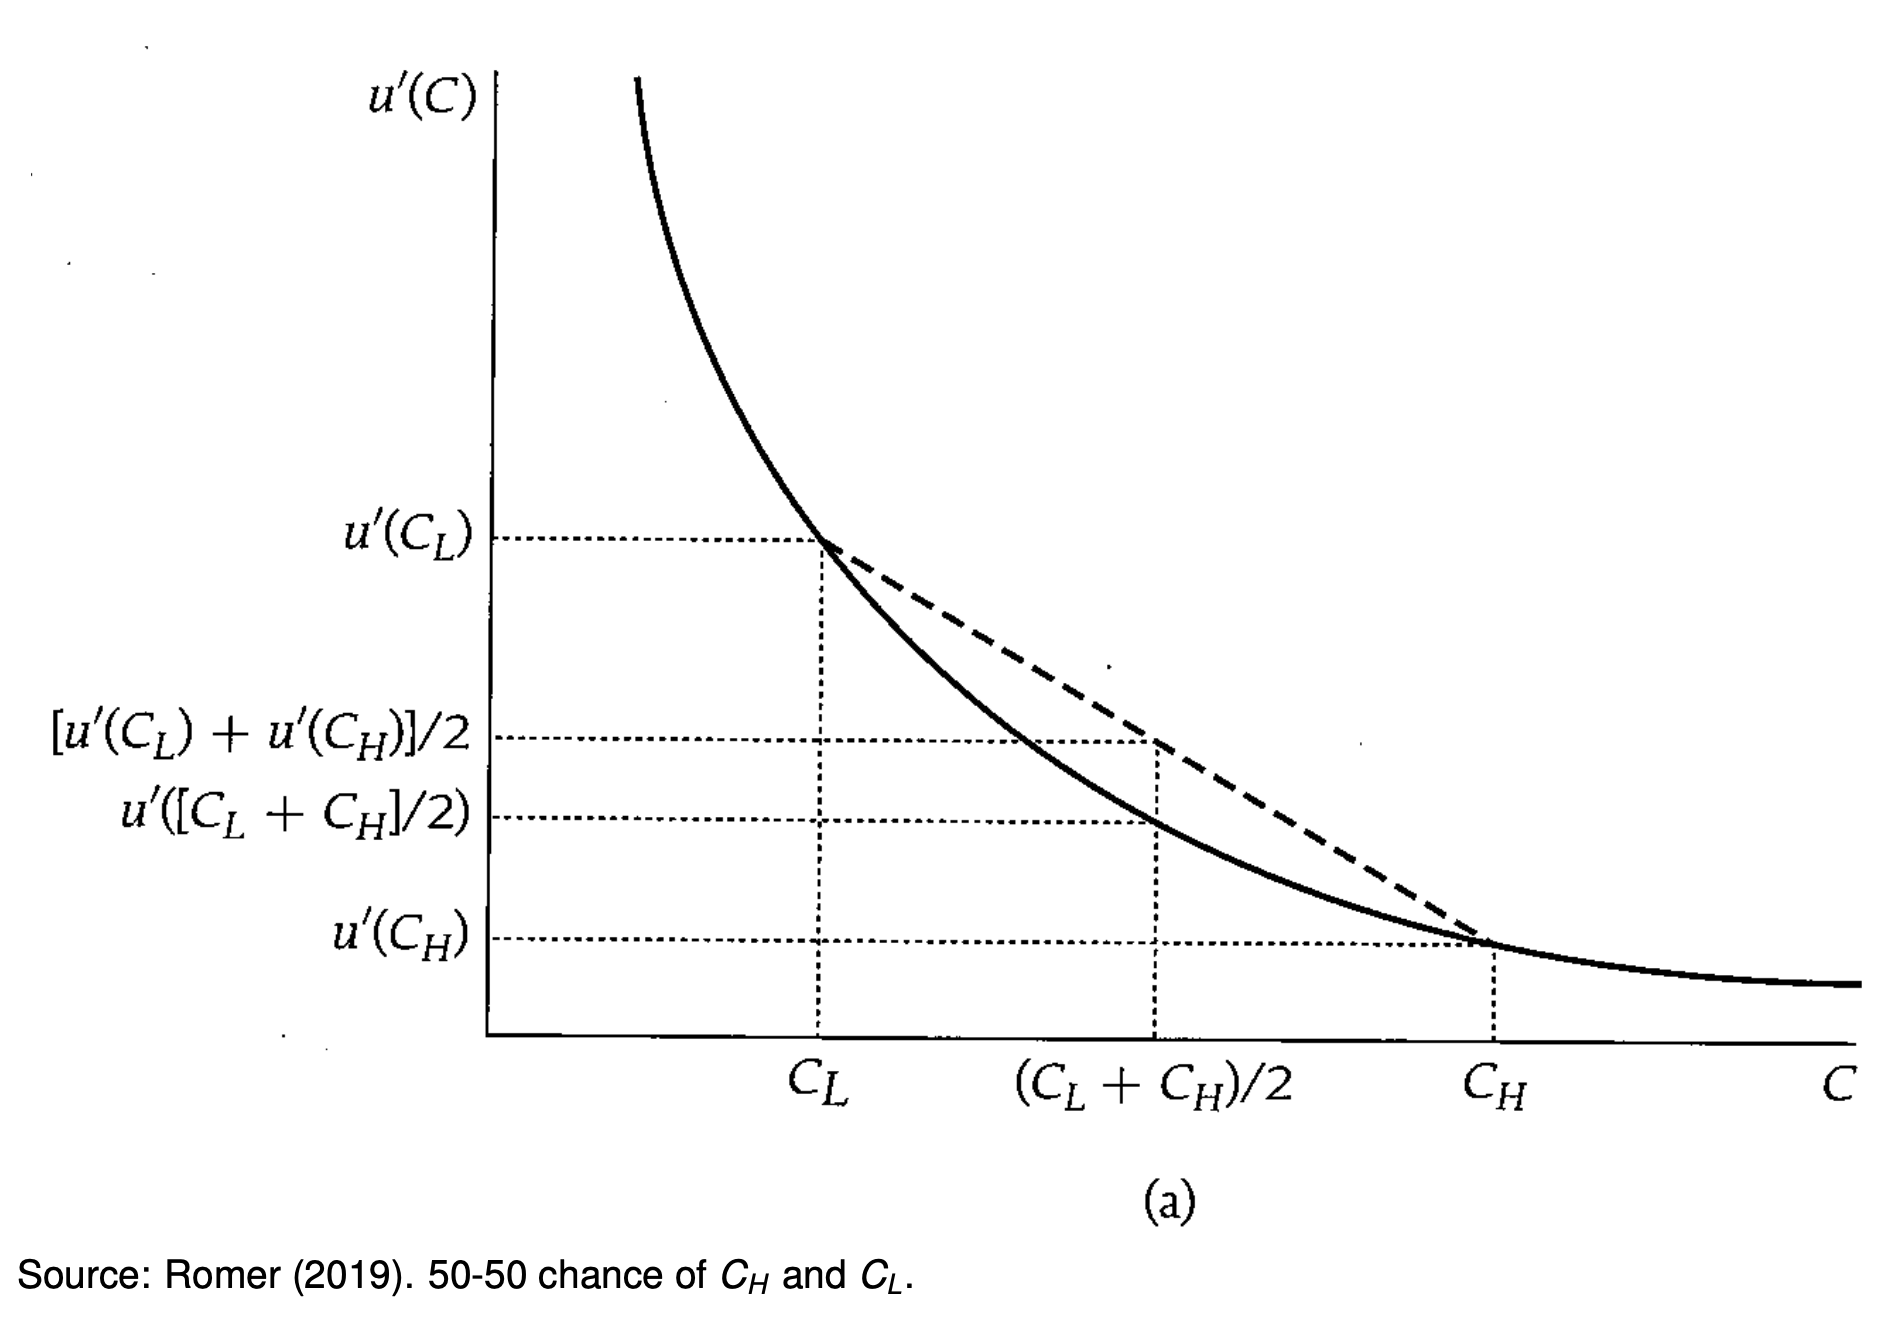
\includegraphics[scale=0.3]{./figures/precautionary}
	\end{figure}
\end{frame}



%%%%%%%%%%%%%%%%%%%%%%%%%%  SLIDE   %%%%%%%%%%%%%%%%%%%%%%%%%%%%%%%%
\begin{frame}{6. Linearizing the Euler Equation}

\begin{witemize}
\item Recall Euler Equation: 
\begin{equation*}
	u'(c_t) = \mathbb E_t \beta R_{t+1} u'(c_{t+1}) 
\end{equation*}

\item Want to transform this equation so it is more amenable to empirical analysis

\item Assume that $R_{t+1}$ is known at time $t$

\item Assume $u$ is isoelastic (i.e., constant relative risk aversion) utility
function, 
\begin{equation*}
	u(c) = \frac{c^{1-\gamma}-1}{1-\gamma}. 
\end{equation*}
(Aside: $\lim_{\gamma \rightarrow 1}\frac{c^{1-\gamma }-1}{1-\gamma }=\ln c$. Important special case.)

\end{witemize}
\end{frame}


%%%%%%%%%%%%%%%%%%%%%%%%%%  SLIDE   %%%%%%%%%%%%%%%%%%%%%%%%%%%%%%%%
\begin{frame}{}

\begin{witemize}
\item Recall $-\log \beta = \rho$ and $\log R_{t+1} = r_{t+1}$

\item Noting that $u'(c) = c^{-\gamma}$, rewrite Euler equation as
\begin{align*}
	c_t^{-\gamma} &= \mathbb E_t \beta R_{t+1} c_{t+1}^{-\gamma} \\
	1 &= \mathbb E_t \exp \Big[\log ( \beta R_{t+1} c_{t+1}^{-\gamma} c_t^\gamma
	)\Big] \\
	1 &= \mathbb E_t \exp \Big[- \rho + r_{t+1} -\gamma \log (c_{t+1} / c_t) \Big] \\
	1 &= \mathbb E_t \exp \Big[r_{t+1} - \rho - \gamma \Delta \log c_{t+1} \Big]
\end{align*}

\end{witemize}
\end{frame}


%%%%%%%%%%%%%%%%%%%%%%%%%%  SLIDE   %%%%%%%%%%%%%%%%%%%%%%%%%%%%%%%%
\begin{frame}{}

\begin{witemize}
\item Assume that $\Delta \log c_{t+1}$\ is conditionally normally distributed. So, 
\begin{equation*}
	1 = \exp \bigg[r_{t+1} - \rho - \gamma \mathbb E_t \Delta \log c_{t+1} + \frac{1}{2} \gamma^2 \mathbb Var_t \Delta \log c_{t+1} \bigg] 
\end{equation*}

\item Taking logs of both sides 
\begin{equation*}
	\mathbb E_t \Delta \log c_{t+1} = \frac{1}{\gamma} (r_{t+1} - \rho) + \frac{\gamma}{2} \mathbb Var_t \Delta \log c_{t+1}. 
\end{equation*}

\item \textbf{Precautionary savings}: $\frac{\gamma}{2} \mathbb Var_t \Delta \log c_{t+1} > 0$ implies positive expected consumption growth. Why?  

\end{witemize}
\end{frame}


%%%%%%%%%%%%%%%%%%%%%%%%%%  SLIDE   %%%%%%%%%%%%%%%%%%%%%%%%%%%%%%%%
\begin{transitionframe}
	{\color{white} \Huge \textbf{Part 2: Empirical Regularities} \vspace{2mm}}
\end{transitionframe}


%%%%%%%%%%%%%%%%%%%%%%%%%%  SLIDE   %%%%%%%%%%%%%%%%%%%%%%%%%%%%%%%%
\begin{frame}{1. Empirical tests of the Euler equation}

\begin{witemize}
\item Recall the consumption Euler equation
\begin{equation*}
	u' (c_t) = \mathbb E_t \beta R_{t+1} u'(c_{t+1}) 
\end{equation*}

\item Rewrite linearized Euler equation in regression form
\begin{equation*}
	\Delta \log c_{t+1} = \frac{1}{\gamma} (r_{t+1} - \rho) + \frac{\gamma}{2} \mathbb Var_t \Delta \log c_{t+1} + \varepsilon_{t+1} 
\end{equation*}
where $\varepsilon_{t+1}$ is orthogonal to any information known at date $t$

\item The conditional variance term is often referred to as the ``precautionary
savings term'' (more on this later)
\end{witemize}
\end{frame}

%%%%%%%%%%%%%%%%%%%%%%%%%%  SLIDE   %%%%%%%%%%%%%%%%%%%%%%%%%%%%%%%%
\begin{frame}{}

\begin{witemize}
\item We sometimes (counterfactually) assume that $\mathbb Var_t \Delta \log c_{t+1}$ is constant (i.e., independent of time). So the Euler equation reduces to: 
\begin{equation*}
	\Delta \log c_{t+1} = \text{constant} + \frac{1}{\gamma} (r_{t+1} - \rho) +\varepsilon_{t+1} 
\end{equation*}

\item When we replace the precautionary term with a constant, we are effectively ignorning its effect (since it is no longer separately identified from the other constant term: $\frac{\rho}{\gamma})$
\end{witemize}
\end{frame}


%%%%%%%%%%%%%%%%%%%%%%%%%%  SLIDE   %%%%%%%%%%%%%%%%%%%%%%%%%%%%%%%%
\begin{frame}{}

\begin{witemize}
\item Hundreds of papers have estimated a linearized Euler equation: 
\begin{equation*}
	\Delta \log c_{t+1} = \text{constant} + \frac{1}{\gamma} r_{t+1} + \beta
X_t + \varepsilon_{t+1} 
\end{equation*}

\item The principal goals of these regressions are twofold:
\end{witemize}

\vspace{6mm}
\begin{enumerate}
\item [1.] Estimate $\frac{1}{\gamma}$, the elasticity of intertemporal substitution (EIS) $=\frac{\partial \Delta \log c_{t+1}}{\partial r_{t+1} }$. For example, see Hall (1988).

\vspace{3mm}
\begin{itemize}
\item For this model, the EIS is the inverse of the CRRA
\end{itemize}

\end{enumerate}
\end{frame}


%%%%%%%%%%%%%%%%%%%%%%%%%%  SLIDE   %%%%%%%%%%%%%%%%%%%%%%%%%%%%%%%%
\begin{frame}{}

\begin{enumerate}
\item[2.] Test the orthogonality restriction: 
\begin{equation*}
	\Big\{ \Omega_t \equiv \text{information set at date} t \Big\} \perp \varepsilon_{t+1} 
\end{equation*}


\begin{itemize}
\item In other words, test the restriction that information available at time $t$ does \textbf{not} predict consumption growth in the following regression
\begin{equation*}
	\Delta \log c_{t+1} = \text{constant} + \frac{1}{\gamma} r_{t+1} + \beta
X_t + \varepsilon_{t+1}
\end{equation*}

\item For example, does the date $t$ expectation of income growth, $\mathbb E_t\Delta \log y_{t+1}$ predict date $t+1$ consumption growth?
\end{itemize}
\end{enumerate}

\end{frame}


%%%%%%%%%%%%%%%%%%%%%%%%%%  SLIDE   %%%%%%%%%%%%%%%%%%%%%%%%%%%%%%%%
\begin{frame}{}

\begin{equation*}
	\Delta \log c_{t+1} = \text{constant} + \frac{1}{\gamma} \mathbb E_t r_{t+1} + \alpha \mathbb E_t \Delta \log y_{t+1} + \varepsilon_{t+1} 
\end{equation*}

\vspace{2mm}
\begin{witemize}
\item Finding: $\hat \alpha \in [0.1, 0.35]$ so $\mathbb E_t \Delta \log y_{t+1}$ covaries with $\Delta \log c_{t+1}$ 

	\vspace{2mm}
	{\footnotesize E.g. Campbell and Mankiw 1989, Shea 1995, Shapiro 2005, Parker and Broda 2014, Gelman, Kariv, Shapiro, Silverman, and Tadelis 2015, Ganong and Noel 2018}

\item Orthogonality restriction is violated: information at date $t$ predicts consumption growth from $t$ to $t+1$

\item In other words, the assumptions (1) the Euler equation is true, (2) the utility function is in the CRRA class, (3) the linearization is accurate, and (4) $\mathbb Var_t \Delta \log c_{t+1}$ is constant, are jointly rejected

	\vspace{1mm}
	{\footnotesize Recall we also assumed households have perfect foresight over $R_{t+1}$}

\end{witemize}
\end{frame}


%%%%%%%%%%%%%%%%%%%%%%%%%%  SLIDE   %%%%%%%%%%%%%%%%%%%%%%%%%%%%%%%%
\begin{frame}{2. How does consumption respond to windfalls?}

\begin{witemize}
\item Related literature estimates the marginal propensity to consume non-durables
(MPC) out of wealth ``windfalls'' (or unearned income)

\begin{equation*}
	c_{t+1} = \text{constant} + \alpha w_{t+1} + \varepsilon_{t+1}
\end{equation*}

\item $\hat \alpha \in [0.1, 0.35]$ so $MPC$ is much higher than in classical models 

	\vspace{2mm}
	{\footnotesize E.g. Havranek and Sokolova 2020, Ganong, Jones, Noel, Greig, Farrell, and Wheat 2020, Parker et al 2013, Kueng 2018, Fagereng et al 2019}

\item Note that marginal propensity for expenditure ($MPX$) is about three times as high as $\hat \alpha$ due to expenditures on durables (Laibson-Maxted-Moll 2022)

\end{witemize}
\end{frame}


%%%%%%%%%%%%%%%%%%%%%%%%%%  SLIDE   %%%%%%%%%%%%%%%%%%%%%%%%%%%%%%%%
\begin{frame}{Why does $\mathbb E_t \Delta \log y_{t+1}$ predict $\Delta \log c_{t+1}$?}

\begin{witemize}
\item Welfare costs of smoothing are second-order (Cochrane 1989, Pischke 1995, Browning and Crossley 2001, Kueng 2015, Gabaix2016)

\item Leisure and consumption expenditure are substitutes (Heckman 1974, Ghez and Becker 1975, Aguiar and Hurst 2005, 2007, Stephens and Toohey 2019)

\item Work-based expenses (see Ganong and Noel 2016)

\item Households support lots of dependents in mid-life when income is highest (Browning 1992, Attanasio 1995, Seshadri et al 2006)

\end{witemize}
\end{frame}

%%%%%%%%%%%%%%%%%%%%%%%%%%  SLIDE   %%%%%%%%%%%%%%%%%%%%%%%%%%%%%%%%
\begin{frame}{Why does $\mathbb E_t \Delta \log y_{t+1}$ predict $\Delta \log c_{t+1}$?}

\begin{witemize}
\item Some consumers use rules of thumb: $c_{it}=\alpha y_{it}$ (Campbell and Mankiw 1989, Thaler and Shefrin 1981, Gabaix 2016)

\item Markets are incomplete, households are impatient, and utiliy is CRRA (Deaton 1991, Carroll 1992): these assumptions make the variance term time-varying ($V_{t}\Delta \ln c_{t+1}$)

\item Markets are incomplete, households are present-biased, and utility is CRRA (Laibson 1997, Harris and Laibson 2001, Shapiro 2005, Laibson, Maxted, Repetto, and Tobacman 2016): these assumptions violate the Euler equation altogether

\end{witemize}
\end{frame}


%%%%%%%%%%%%%%%%%%%%%%%%%%  SLIDE   %%%%%%%%%%%%%%%%%%%%%%%%%%%%%%%%
\begin{transitionframe}
	{\color{white} \huge \textbf{Part 3: Tractable Models of Consumption} \vspace{2mm}}
\end{transitionframe}


%%%%%%%%%%%%%%%%%%%%%%%%%%  SLIDE   %%%%%%%%%%%%%%%%%%%%%%%%%%%%%%%%
\begin{frame}{What's the goal in this part of the lecture?}
\begin{witemize}
\item Start with simplest model of consumption and add ingredients one by one

\item Each model admits closed-form solution $\to$ illustrates economic mechanism

	{\footnotesize Closed-form solutions are rare and special. CT does a lot of work here!}

\item We will study 3 crucial extensions to simplest model:
\begin{enumerate}
	\item Labor supply
	\item Precautionary savings
	\item Incomplete markets and liquidity constraints
\end{enumerate}

\item By the end, we arrive at \textbf{the canonical consumption model}
\end{witemize}
\end{frame}


%%%%%%%%%%%%%%%%%%%%%%%%%%  SLIDE   %%%%%%%%%%%%%%%%%%%%%%%%%%%%%%%%
\begin{frame}{1. Eat-the-pie: no risk, no income}
\begin{witemize}
\item Already saw variant of this in DT $\to$ even more tractable with CT! 

\item Time is continuous, $t \in [0, \infty)$

\item Infinitely-lived household's wealth evolves according to 
\begin{equation*}
	\dot a = ra - c
\end{equation*}
given initial wealth position $a_0$, constant interest rate $r$

\item The HJB equation is given by
\begin{equation*}
	\rho V(a) = \frac{1}{1-\gamma} c(a)^{1-\gamma} + V_a (r a - c(a))
\end{equation*}
where $c(a)$ solves first-order condition $c(a)^{-\gamma} = V_a$
\end{witemize}
\end{frame}


%%%%%%%%%%%%%%%%%%%%%%%%%%  SLIDE   %%%%%%%%%%%%%%%%%%%%%%%%%%%%%%%%
\begin{frame}{}
\begin{witemize}
\item Consider Ansatz $V = Aa^B$, so that $V_a = AB a^{B-1}$ and $c = [AB a^{B-1}]^{- \frac{1}{\gamma}}$

\item Then HJB becomes
\begin{align*}
	\rho A a^B &= \frac{1}{\gamma} \bigg( [AB a^{B-1}]^{- \frac{1}{\gamma}} \bigg)^{1-\gamma} + AB a^{B-1} \bigg( r a - [AB a^{B-1}]^{- \frac{1}{\gamma}} \bigg) \\
	\rho A a^B - r A B a^B &= \frac{\gamma}{1-\gamma} [A B a^{B-1}]^\frac{\gamma-1}{\gamma}
\end{align*}
Plug in $B = 1-\gamma$ and solve for (do this yourself!)
\begin{equation*}
	A = \frac{1}{1-\gamma} \bigg[ \frac{1}{\gamma} \rho - \frac{1-\gamma}{\gamma} r \bigg]^{-\gamma}
\end{equation*}

\item Solution of this model:
\begin{align*}
	V(a) = \frac{1}{1-\gamma} \kappa^{-\gamma} a^{1-\gamma}
	\quad \text{ and } \quad
	V_a(a) = \kappa^{-\gamma} a^{-\gamma} 
	\quad \text{ and } \quad
	c(a) = \kappa a
\end{align*}
\end{witemize}
\end{frame}


%%%%%%%%%%%%%%%%%%%%%%%%%%  SLIDE   %%%%%%%%%%%%%%%%%%%%%%%%%%%%%%%%
\begin{frame}{}
\begin{witemize}
\item Marginal propensity to consume (MPC) is defined as
\begin{equation*}
	c'(a) = \kappa \equiv \frac{1}{\gamma} \rho - \frac{1-\gamma}{\gamma} r
\end{equation*}

\item Consider $u(c) = \log(c)$, with $\gamma \to 1$ (income and substitution effects offset each other)
\begin{equation*}
	c'(a) = \kappa = \rho \approx 5 \% \text{ annually }
\end{equation*}

\item The standard CRRA calibration with $\gamma = 2$ yields
\begin{equation*}
	c'(a) = \kappa \equiv \frac{1}{2} (\rho + r).
\end{equation*}
In models with uninsurable risk and incomplete financial markets, $r < \rho$

\end{witemize}
\end{frame}


%%%%%%%%%%%%%%%%%%%%%%%%%%  SLIDE   %%%%%%%%%%%%%%%%%%%%%%%%%%%%%%%%
\begin{frame}{}

What you should take away from this: In the simplest model of consumption 

\vspace{4mm}
\begin{enumerate}
\item The consumption policy function is linear: $c(a) = \kappa a$

\item MCP is small, $\kappa \approx 5\%$

\item MPC does not vary with wealth or income
\end{enumerate}

\vspace{4mm}
These predictions are strongly rejected in the data!

\vspace{6mm}
\textbf{Q:} Is there a better theory of consumption consistent with MPCs that (i) are large and (ii) vary with wealth / income?
\end{frame}


%%%%%%%%%%%%%%%%%%%%%%%%%%  SLIDE   %%%%%%%%%%%%%%%%%%%%%%%%%%%%%%%%
\begin{frame}{2. What happens when we add (unearned) income?}

\begin{witemize}
\item Household now earns exogenous income $w$ and wealth evolves as
\begin{equation*}
	\dot a = ra + w - c
\end{equation*}

\item HJB equation becomes
\begin{equation*}
	\rho V(a) = \frac{1}{1-\gamma} c(a)^{1-\gamma} + V_a (r a + w - c(a))
\end{equation*}

\item Solution of this model (work this out yourself):
\begin{align*}
	V(a) = \frac{1}{1-\gamma} \kappa^{-\gamma} \Big( a + \frac{w}{r} \Big)^{1-\gamma} 
	\quad \text{ and } \quad
	c(a) = \kappa \Big(a + \frac{w}{r} \Big)
\end{align*}
with MPC given by: $c'(a) = \kappa$ (as before)

\item Intuition? Human capital affects lifetime wealth but not MPC
\end{witemize}
\end{frame}


%%%%%%%%%%%%%%%%%%%%%%%%%%  SLIDE   %%%%%%%%%%%%%%%%%%%%%%%%%%%%%%%%
\begin{frame}{3. What happens with a labor supply decision?} 

\begin{witemize}
\item Households solve: $\max \int_0^\infty e^{- \rho t} u(c_t, h_t) dt$, with $u(c, h) = \frac{1}{1-\gamma} (c - \frac{h^{1+\eta}}{1+\eta})^{1-\gamma}$ (GHH)
\begin{align*}
	\rho V(a) = \max_{c, h} \Big\{ u(c, h) + (r a + w h - c) \partial_a V(a) \Big\}
\end{align*}
where FOCs are $u_c = V_a$ and $u_h = - w V_a$, so 
\begin{align*}
	\bigg( c - \frac{h^{1+\eta}}{1+\eta} \bigg)^{-\gamma} = V_a 
	\quad \text{ and } \quad
	\bigg( c - \frac{h^{1+\eta}}{1+\eta} \bigg)^{-\gamma} h^\eta = w V_a
\end{align*}

\item Putting FOCs together, $c = V_a^{- \frac{1}{\gamma}} + \frac{1}{1 + \eta} w^\frac{1+\eta}{\eta}$ and $h = w^\frac{1}{\eta}$

\item Intuition: under GHH there is no income effect on labor supply
\end{witemize}
\end{frame}


%%%%%%%%%%%%%%%%%%%%%%%%%%  SLIDE   %%%%%%%%%%%%%%%%%%%%%%%%%%%%%%%%
\begin{frame}{}
\begin{witemize}
\item HJB becomes
\begin{align*}
	\rho V &= \frac{1}{1-\gamma} V_a^\frac{\gamma-1}{\gamma} + V_a \Big( ra + w h - c \Big) \\
	&= \frac{1}{\gamma} V_a^\frac{\gamma-1}{\gamma} + V_a \bigg( ra + \frac{\eta}{1 + \eta} w^\frac{1+\eta}{\eta} - V_a^{- \frac{1}{\gamma}} \bigg)
\end{align*}

\item Solution of this model given by (work this out yourself):
\begin{align*}
	V(a) &= \frac{1}{1-\gamma} \kappa^{-\gamma} \bigg( a + \frac{\eta}{1+\eta} \frac{w^\frac{1+\eta}{\eta}}{r} \bigg)^{1-\gamma}
\end{align*}
implying
\begin{align*}
	V'(a) &= \kappa^{-\gamma} \bigg( a + \frac{\eta}{1+\eta} \frac{w^\frac{1+\eta}{\eta}}{r} \bigg)^{-\gamma} \\
	c(a) &= \kappa a + \bigg( \frac{\eta}{1+\eta} \frac{\tilde \kappa}{r} + \frac{1}{1+\eta} \bigg) w^\frac{1+\eta}{\eta}
\end{align*}
\end{witemize}
\end{frame}


%%%%%%%%%%%%%%%%%%%%%%%%%%  SLIDE   %%%%%%%%%%%%%%%%%%%%%%%%%%%%%%%%
\begin{frame}{}
\begin{witemize}
\item The household's MPC (out of wealth) is still constant and given by $c'(a) = \text{MPC} = \kappa$ (same $\kappa$ as before)

\item Intuition: we correct for an \textit{effective wage adjustment} in human capital / lifetime wealth but consumption is unaffected by labor supply under GHH

\item This is because GHH shuts down income effects on labor supply

\end{witemize}
\end{frame}




%%%%%%%%%%%%%%%%%%%%%%%%%%  SLIDE   %%%%%%%%%%%%%%%%%%%%%%%%%%%%%%%%
\begin{frame}{4. Precautionary savings I: return risk}
\begin{witemize}
\item In the data, we see (a) much higher MPCs and (b) MPCs are higher at low income / wealth

\item So far: we considered deterministic consumption-savings problems. They all yielded (roughly) $\text{MPC} \approx \rho \approx 5\%$ annually. 

\item We now start exploring theories of consumption that can break this and match the data much better

\item Let's start with a simple example of return risk: You can only trade stocks (no bonds) and stocks trade at a stochastic price
\begin{equation*}
	Q dk = Dk - c
\end{equation*}
where $D$ is the dividend
\end{witemize}
\end{frame}


%%%%%%%%%%%%%%%%%%%%%%%%%%  SLIDE   %%%%%%%%%%%%%%%%%%%%%%%%%%%%%%%%
\begin{frame}{}
\begin{witemize}
\item Define net worth as $a = Qk$, so $da = k dQ + Q dk$ by Ito's product rule, noting that $(dk)(dQ) = 0$, so 
\begin{equation*}
	da = \frac{D}{Q} - c + a \frac{dQ}{Q}
\end{equation*}

\item Assume stock prices follow a diffusion process (geometric Brownian): 
\begin{equation*}
	\frac{dQ}{Q} = \mu dt + \sigma dB
\end{equation*}

\item Rewrite wealth as: $da = (\mu_R - c) dt + a \sigma dB$, where $\mu_R = \mu_Q + \frac{D}{Q}$ (dividend + capital gains yield)

\item HJB: 
\begin{equation*}
	\rho V(a) = u(c(a) + V_a (\mu_R a - c) + \frac{1}{2} (a \sigma)^2 V_{aa}
\end{equation*}
\end{witemize}
\end{frame}



%%%%%%%%%%%%%%%%%%%%%%%%%%  SLIDE   %%%%%%%%%%%%%%%%%%%%%%%%%%%%%%%%
\begin{frame}{}
\begin{witemize}
\item Solution of this model is (work this out yourself): 
\begin{align*}
	V(a) &= \frac{1}{1-\gamma} \tilde \kappa^{-\gamma} a^{1-\gamma} \\
	c(a) &= \tilde \kappa a,
\end{align*}
where 
\begin{equation*}
	\kappa \equiv \frac{1}{\gamma} \bigg[ \rho - (1-\gamma) \mu_R + \underbrace{ \gamma(1-\gamma) \frac{\sigma^2}{2}}_\text{Precautionary savings} \bigg] 
\end{equation*}

\item Households' MPC now has a precautionary savings term $\frac{1}{2}(1-\gamma) \sigma^2$

\item The consumption Euler equation for this model (work this out yourself) is:
\begin{equation*}
	\mathbb{E} \bigg( \frac{dc}{c} \bigg) = \frac{r - \rho}{\gamma} dt - \frac{1-\gamma}{2} \sigma^2 dt
\end{equation*}

\item For $\gamma = 2$, precautionary term is negative, so households tilt consumption profile towards the future (hence, precautionary savings)
\end{witemize}
\end{frame}



%%%%%%%%%%%%%%%%%%%%%%%%%%  SLIDE   %%%%%%%%%%%%%%%%%%%%%%%%%%%%%%%%
\begin{transitionframe}
	{\color{white} \Huge \textbf{Part 4: Liquidity Constraints} \vspace{2mm}}
\end{transitionframe}


%%%%%%%%%%%%%%%%%%%%%%%%%%  SLIDE   %%%%%%%%%%%%%%%%%%%%%%%%%%%%%%%%
\begin{frame}{}
\begin{witemize}
\item We now work through arguably \textit{the} benchmark model of consumption in macro

\item Household faces (1) uninsurable income risk and (2) a borrowing constraint 

\item Capture income risk via stochastic process $\{z_t\}$ 

\item Household can trade a bond, $a_t$, but subject to constraint $a_t \geq \underline a$
\end{witemize}

\vspace{6mm}
\textbf{Sequence problem}:
\begin{equation*}
	V_0 = \max_{ \{ c_t \}_{t \geq 0} } \mathbb{E}_0 \int_0^\infty e^{- \rho t} u(c_t) dt
\end{equation*}
\begin{align*}
	da_t &= r a_t + e^{z_t} - c_t \\
	a_t &\geq \underline a \\
	dz_t &= - \theta z_t dt + \sigma dB_t
\end{align*}
\end{frame}


%%%%%%%%%%%%%%%%%%%%%%%%%%  SLIDE   %%%%%%%%%%%%%%%%%%%%%%%%%%%%%%%%
\begin{frame}{}
\begin{witemize}
\item Household states are $(a, z)$, so recursive representation is 
\begin{equation*}
	\rho V = u(c) + (r a + e^z - c) V_a - \theta z V_z + \frac{\sigma^2}{2} V_{zz}
\end{equation*}

% \item First step in deriving Euler equation: envelope condition
% \begin{equation*}
% 	(\rho - r) V_a = (ra + e^z - c) V_{aa} - \theta z V_{z a} + \frac{\sigma^2}{2} V_{zz a }
% \end{equation*}
% 
% \item Using Ito's lemma, noting $V_a$ is function of $(a_t, z_t)$, 
% \begin{align*}
% 	dV_a &= V_{aa} da + V_{az} dz + \frac{1}{2} V_{azz} (dz)^2 \\
% 	&= V_{aa} (r a + e^z - c) dt + V_{az} (- \theta z dt + \sigma dB) + \frac{\sigma^2}{2} V_{azz} dt \\
% 	&= (\rho - r)V_a dt +  \sigma V_{az} dB
% \end{align*}
% \end{witemize}
% \end{frame}
% 
% 
% %%%%%%%%%%%%%%%%%%%%%%%%%%  SLIDE   %%%%%%%%%%%%%%%%%%%%%%%%%%%%%%%%
% \begin{frame}{}
% \begin{witemize}
% \item Using $u_c = V_a$ and $V_{az} = u_{cc} c_z$, Euler equation for marginal utility is
% \begin{equation*}
% 	\frac{du_c}{u_c} = (\rho - r) dt + \sigma \frac{u_{cc} c_z}{u_c} dB
% \end{equation*}
% 
% \item For isoelastic (CRRA), we have $\frac{u_{cc}}{u_c} = - \frac{\gamma}{c}$

\item Consumption Euler equation for CRRA (derivation on Homework):
\begin{equation*}
	\frac{dc}{c} = \frac{r - \rho}{\gamma} dt + \frac{1+\gamma}{2} \bigg( \frac{\sigma c_z}{c} \bigg)^2 dt + \frac{c_z}{c} \sigma dB,
\end{equation*}
where $c_z$ is $\approx$ the marginal propensity out of income shocks

\item The term $ \frac{1+\gamma}{2} \big( \frac{\sigma c_z}{c} \big)^2$ captures a precautionary savings motive due to uncertainty about future income fluctuations (that are not insurable)

\item Where does the borrowing constraint show up here??? $\to$ continuous time!
\end{witemize}
\end{frame}


%%%%%%%%%%%%%%%%%%%%%%%%%%  SLIDE   %%%%%%%%%%%%%%%%%%%%%%%%%%%%%%%%
\begin{frame}{}
	\begin{figure}
		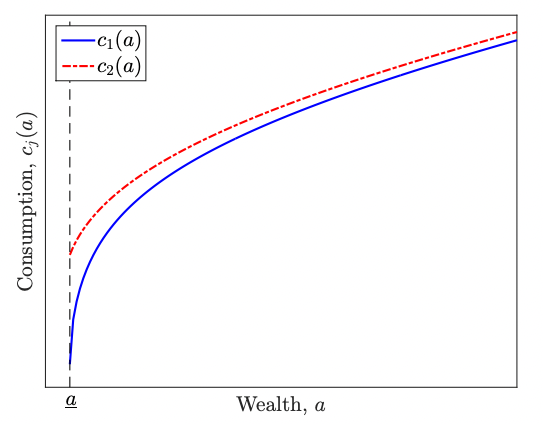
\includegraphics[scale=0.35]{./figures/HACT_consumption}
		\qquad
		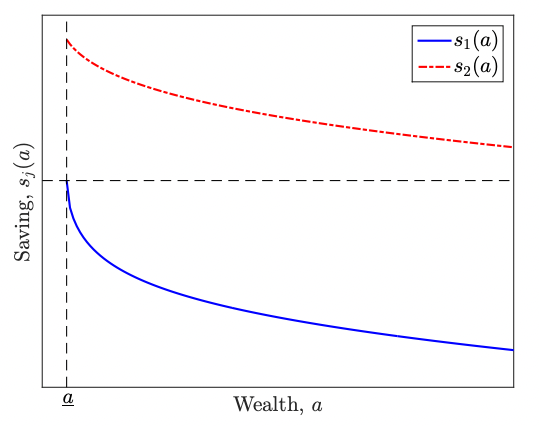
\includegraphics[scale=0.35]{./figures/HACT_savings}
	\end{figure}
\end{frame}


%%%%%%%%%%%%%%%%%%%%%%%%%%  SLIDE   %%%%%%%%%%%%%%%%%%%%%%%%%%%%%%%%
\begin{frame}{Predictions}

\begin{witemize}
\item The consumption function is concave $\to$ MPC varies with wealth

\item Consumption function becomes steep at the borrowing constraint $\to$ low-wealth households have large MPCs

\item Consumption tracks income $\to$ $\Delta \log y_{t+1}$ predicts $\Delta \log c_{t+1}$

\item Households save to build up ``buffer stock'' to smooth income fluctuations 
\end{witemize}
\end{frame}



\end{document}
